\subsection{Voltage Divider Bias Circuit:}

The circuit of Figure 3.2.0 were simulated with two different {\bfseries\itshape NPN} transistors, sames used in the laboratory, this to compare the development results with the simulated. and also, with the theoretical results in section 3.5.

{\bfseries\itshape
\begin{itemize}
\item Simulation of a Voltage Divider Bias Circuit implementing a 2N2222A transistor:
\end{itemize}}

\begin{multicols}{2}
\begin{figure}[H]
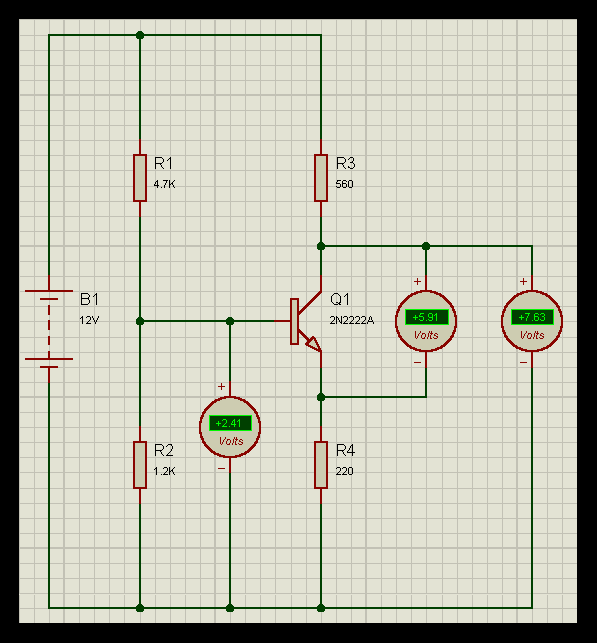
\includegraphics[width = 8cm, height = 10cm]{DVC-2N2222A-Voltage.png}
\centering \linebreak \linebreak Figure 4.1.0: Simulated voltage measures.
\end{figure}

\begin{figure}[H]
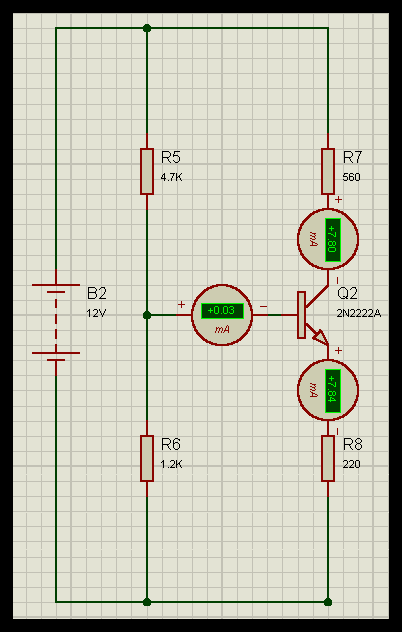
\includegraphics[width = 6cm, height = 10cm]{DVC-2N2222A-Current.png}
\centering \linebreak \linebreak Figure 4.1.1: Simulated current measures.
\end{figure}
\end{multicols}

\begin{center}
\begin{tabular}[1.5cm]{c c c}
\toprule
\toprule
\centering \hspace{220pt} & \hspace{80pt} {\bfseries 2N2222A} \hspace{80pt} & \\
\midrule
\midrule
$V_{B}$ & 2.41 V \\
\cmidrule{1-3}
$V_{C}$ & 7.63 V \\
\cmidrule{1-3}
$V_{CE}$ & 5.91 V \\
\cmidrule{1-3}
$I_{B}$ & 3 $\mu$A \\
\cmidrule{1-3}
$I_{C}$ & 7.8 mA \\
\cmidrule{1-3}
$I_{E}$ & 7.84 mA \\
\bottomrule
\linebreak
\end{tabular}
\linebreak Table 5: Values for simulations in Figures 4.1.0 and 4.1.1.
\end{center}

\pagebreak

{\bfseries\itshape
\begin{itemize}
\item Simulation of a Voltage Divider Bias Circuit implementing a BC547 transistor:
\end{itemize}}

\begin{multicols}{2}
\begin{figure}[H]
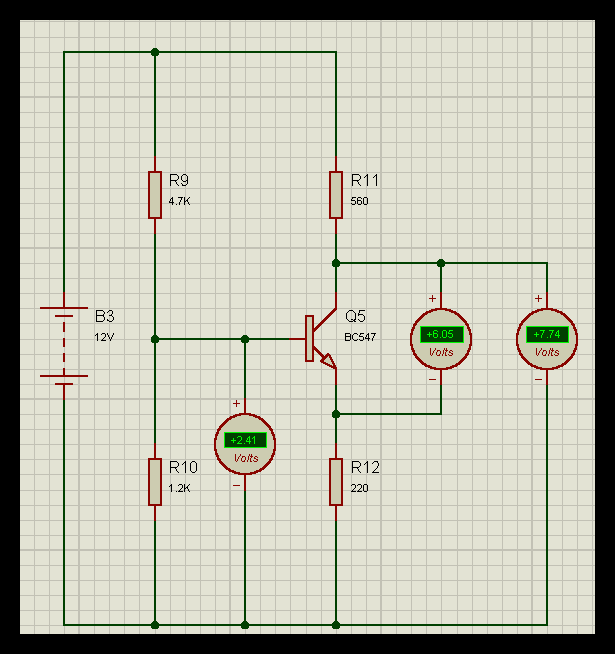
\includegraphics[width = 8cm, height = 10cm]{DVC-BC547-Voltage.png}
\centering \linebreak \linebreak Figure 4.1.2: Simulated voltage measures.
\end{figure}

\begin{figure}[H]
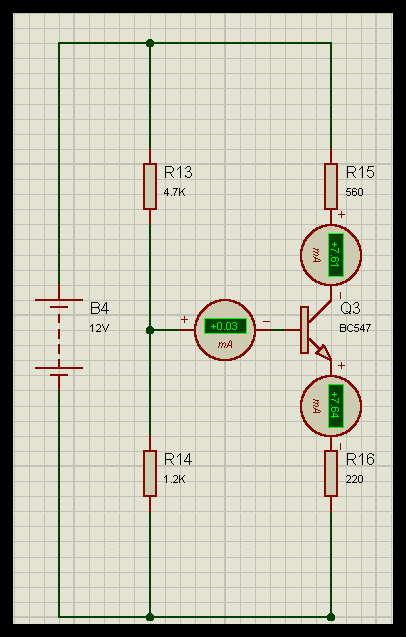
\includegraphics[width = 6cm, height = 10cm]{DVC-BC547-Current.png}
\centering \linebreak \linebreak Figure 4.1.3: Simulated current measures.
\end{figure}
\end{multicols}

\begin{center}
\begin{tabular}[1.5cm]{c c c}
\toprule
\toprule
\centering \hspace{220pt} & \hspace{80pt} {\bfseries BC547} \hspace{80pt} & \\
\midrule
\midrule
$V_{B}$ & 2.41 V \\
\cmidrule{1-3}
$V_{C}$ & 7.74 V \\
\cmidrule{1-3}
$V_{CE}$ & 6.05 V \\
\cmidrule{1-3}
$I_{B}$ & 3 $\mu$A \\
\cmidrule{1-3}
$I_{C}$ & 7.61 mA \\
\cmidrule{1-3}
$I_{E}$ & 7.64 mA \\
\bottomrule
\linebreak
\end{tabular}
\linebreak Table 6: Values for simulations in Figures 4.1.2 and 4.1.3.
\end{center}

\pagebreak